\documentclass[conference]{IEEEtran}
\IEEEoverridecommandlockouts
% The preceding line is only needed to identify funding in the first footnote. If that is unneeded, please comment it out.
\usepackage{cite}
\usepackage{amsmath,amssymb,amsfonts}
\usepackage{algorithm}
\usepackage{algorithmic}
\usepackage{graphicx}
\usepackage{textcomp}
\usepackage{xcolor}


\def\BibTeX{{\rm B\kern-.05em{\sc i\kern-.025em b}\kern-.08em
    T\kern-.1667em\lower.7ex\hbox{E}\kern-.125emX}}
\begin{document}

\begin{algorithm}
\caption{Algorithm: Collaborative Training}
\label{alg:A}
\begin{algorithmic}
\STATE {set $PFCij = proofC (C(Gij ); Gij , rj ; PKj )$} 
\REPEAT 
\STATE set $ Upload masked training results C(Gij ) along with proofs$ 
\REPEAT
\STATE set $Report incorrect C(Gij ) along with PFCij ,PKj to
FLChain, get reward and compensation$ 
\UNTIL{ Unmask aggregation result with sj and get unmasked share
CDij , generate proof} 
\UNTIL{Report incorrect CDij with v, vij ,PFDij ,PKj}
\end{algorithmic}
\end{algorithm}













\begin{table}
\centering
\caption{test table}
\begin{tabular}{|r|r|r|}
\hline
name & class & id \\
\hline
hejian & 2102 & 214712277 \\
\hline
\end{tabular}

\end{table}

\begin{figure}[ht!]
\centering
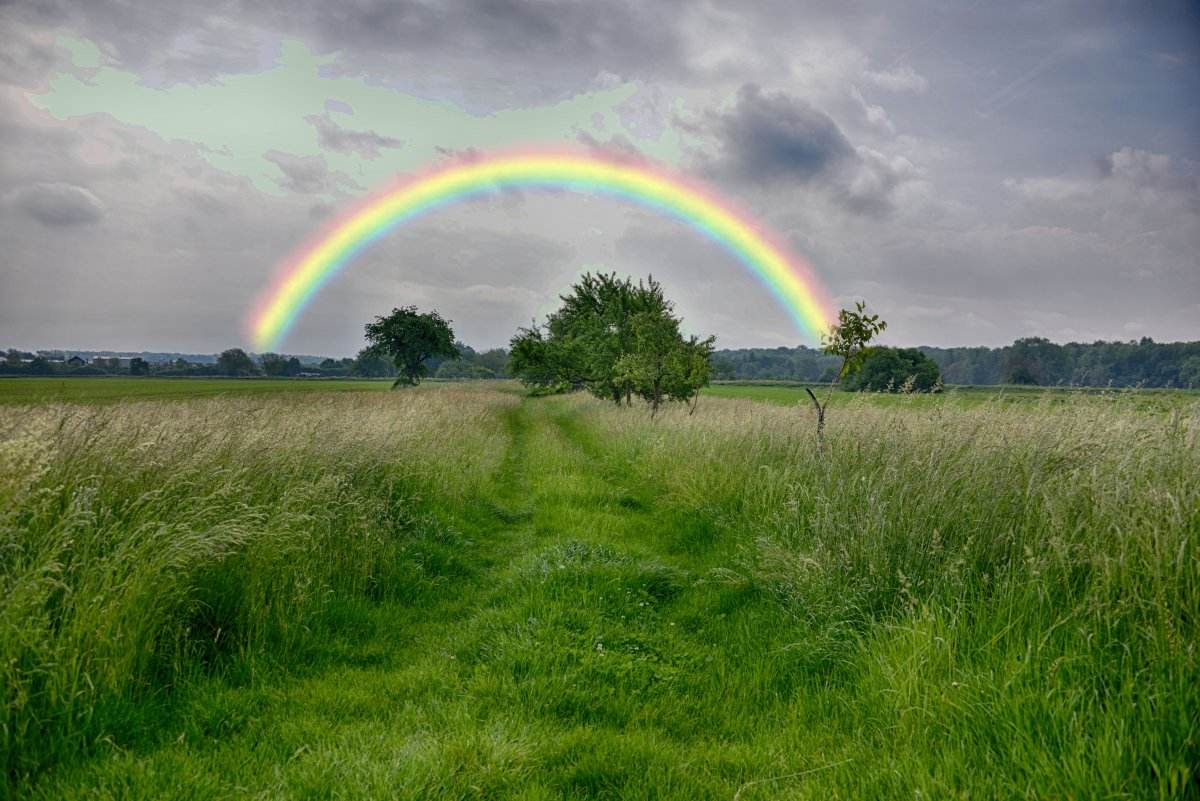
\includegraphics[width=90mm]{234.jpg}
\caption{A simple caption \label{figure-sample}}

\end{figure}


\begin{thebibliography}{00}
\bibitem{b1}  Lampos V , Miller A C , Crossan S , et al. Advances in nowcasting
influenza-like illness rates using search query logs[J]. Scientific Reports,
2015, 5(1):12760.
\end{thebibliography}








\end{document}
